% ------------------------------------------------------------------------------
% TYPO3 Version 9.4 - What's New (Dutch Version)
%
% @license	Creative Commons BY-NC-SA 3.0
% @link		https://typo3.org/help/documentation/whats-new/
% @language	Dutch
% ------------------------------------------------------------------------------

\documentclass[t]{beamer}

% suppress navigation bar
\beamertemplatenavigationsymbolsempty

\mode<presentation>
{
	\usetheme{typo3slides}
}

% global variables
\title{TYPO3 Versie 9.4 - What's New}
\subtitle{Samenvatting van de nieuwe functies, wijzigingen en verbeteringen}
\author{
	\centerline{Gemaakt door:}
	\centerline{Michael Schams}
}

\date{\today}

\begin{document}

% select TYPO3 Share font
\sharefont

% ------------------------------------------------------------------------------
% Title Page
% ------------------------------------------------------------------------------

\begingroup
	\setbeamercolor{normal text}{fg=white,bg=typo3orange}
	\setbeamercolor{title}{fg=white}
	\setbeamercolor{author}{fg=white}
	\setbeamertemplate{footline}[default]
	\begin{frame}
		\titlepage
	\end{frame}
\endgroup

% ------------------------------------------------------------------------------
% Table of Contents
% ------------------------------------------------------------------------------

\section*{TYPO3 Versie 9.4 - What's New}
\begin{frame}[fragile]
	\frametitle{Inhoudsopgave}
	\framesubtitle{Inhoudsopgave}

	\tableofcontents

\end{frame}

% ------------------------------------------------------------------------------

% ------------------------------------------------------------------------------
% TYPO3 Version 9.2 - What's New - Chapter "Introduction" (English Version)
%
% @author	Michael Schams <schams.net>
% @license	Creative Commons BY-NC-SA 3.0
% @link		http://typo3.org/download/release-notes/whats-new/
% @language	English
% ------------------------------------------------------------------------------
% LTXE-CHAPTER-UID:		7fdf26cc-362160ab-d6c8b905-19722b20
% LTXE-CHAPTER-NAME:	Introduction
% ------------------------------------------------------------------------------

\section{Einführung}
\begin{frame}[fragile]
	\frametitle{Einführung}

	\begin{center}\huge{Einführung}\end{center}
	\begin{center}\huge{\color{typo3darkgrey}\textbf{Fakten}}\end{center}

\end{frame}

% ------------------------------------------------------------------------------
% LTXE-SLIDE-START
% LTXE-SLIDE-UID:		3214e510-8ceda314-7689e14c-2d422661
% LTXE-SLIDE-TITLE:		TYPO3 Version 9.2 - The Facts
% ------------------------------------------------------------------------------
\begin{frame}[fragile]
	\frametitle{Einführung}
	\framesubtitle{TYPO3 Version 9.2 - Fakten}

	\begin{itemize}
		\item Veröffentlichungsdatum: 10. April 2018
		\item Releasetyp: Sprint Release
	\end{itemize}

	\begin{figure}
		
\includegraphics[width=0.95\linewidth]{Introduction/typo3-v92-banner.jpg}
	\end{figure}

\end{frame}

% ------------------------------------------------------------------------------
% LTXE-SLIDE-START
% LTXE-SLIDE-UID:		9919ea87-1d45cce7-36a77e6a-ca0598c2
% LTXE-SLIDE-TITLE:		System Requirements
% ------------------------------------------------------------------------------
\begin{frame}[fragile]
	\frametitle{Einführung}
	\framesubtitle{Systemvoraussetzungen}

	\begin{itemize}
		\item PHP Version 7.2\newline
			\smaller
				(wird möglicherweise für zukünftige Versionen auf PHP 7.1 oder 7.0 herabgesetzt)
			\normalsize

		\item PHP Einstellungen:

			\begin{itemize}
				\item \texttt{memory\_limit} >= 128M
				\item \texttt{max\_execution\_time} >= 240s
				\item \texttt{max\_input\_vars} >= 1500
				\item compilation option \texttt{-}\texttt{-disable-ipv6} must \underline{not} be used
			\end{itemize}

		\item Die meisten von \textbf{Doctrine DBAL} unterstützten Datenbankserver arbeiten auch mit TYPO3.
			Getestete DB-Engines sind zum Beispiel:
	\end{itemize}

	\begin{figure}
		
\includegraphics[width=0.70\linewidth]{Introduction/logo-databases.png}
	\end{figure}

\end{frame}

% ------------------------------------------------------------------------------
% LTXE-SLIDE-START
% LTXE-SLIDE-UID:		35a15406-7f01d16c-e43a8668-7294e2be
% LTXE-SLIDE-TITLE:		Development, Release and Maintenance Timeline
% ------------------------------------------------------------------------------
\begin{frame}[fragile]
	\frametitle{Einführung}
	\framesubtitle{Entwicklung, Veröffentlichung und Instandhaltung}

	\textbf{TYPO3 v9}

	\begin{figure}
		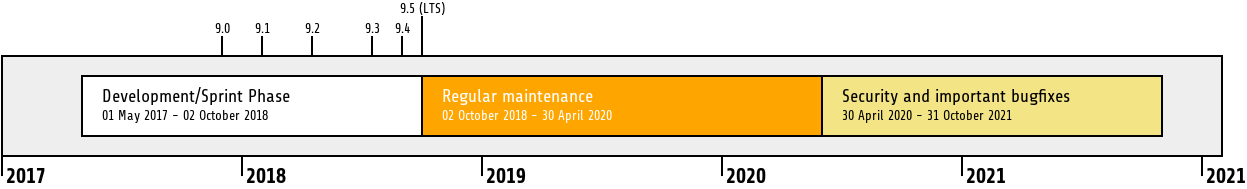
\includegraphics[width=1\linewidth]{Introduction/typo3-v9-lifecycle.png}
	\end{figure}

	\textbf{Erweiterte Unterstützung}\newline
	\smaller
		Die \href{https://typo3.com}{TYPO3 GmbH} bietet weitere Supportmöglichkeiten
		für TYPO3 v9 LTS auch nach dem 31. October 2021 für bis zu zwei weitere Jahre.
	\normalsize

%	\url{https://typo3.com/our-services/extended-support/}

\end{frame}

% ------------------------------------------------------------------------------
% LTXE-SLIDE-START
% LTXE-SLIDE-UID:		0b847921-4c7fdd13-d90d4a71-f6b1ea3a
% LTXE-SLIDE-TITLE:		TYPO3 v9 Roadmap
% ------------------------------------------------------------------------------
\begin{frame}[fragile]
	\frametitle{Einführung}
	\framesubtitle{TYPO3 v9 Roadmap}

	Voraussichtliche Veröffentlichungen und deren Hauptfokus:

	\begin{itemize}

		\item v9.0 \tabto{1.1cm}12/Dec/2017\tabto{3.4cm}Install Tool and Page Tree Refactoring,\newline
			\tabto{3.4cm}Vereinheitlichte Seitenübersetzungen
		\item v9.1 \tabto{1.1cm}30/Jan/2018\tabto{3.4cm}Redirect Handling
		\item
			\begingroup
				\color{typo3orange}
					v9.2 \tabto{1.1cm}10/Apr/2018\tabto{3.4cm}Site Configuration
			\endgroup
		\item v9.3 \tabto{1.1cm}12/Jun/2018\tabto{3.4cm}URL Routing 
		\item v9.4 \tabto{1.1cm}04/Sep/2018\tabto{3.4cm}Frontend Editing (Feature Freeze)
		\item v9.5 \tabto{1.1cm}02/Oct/2018\tabto{3.4cm}LTS Release

	\end{itemize}

	\smaller
		\url{https://typo3.org/news/article/typo3-v9-roadmap/}\newline
		\url{https://typo3.org/typo3-cms/roadmap/}
	\normalsize

\end{frame}

% ------------------------------------------------------------------------------
% LTXE-SLIDE-START
% LTXE-SLIDE-UID:		f1dbd9af-b7f82720-a1ae1511-544f2f94
% LTXE-SLIDE-TITLE:		Installation
% ------------------------------------------------------------------------------
\begin{frame}[fragile]
	\frametitle{Einführung}
	\framesubtitle{Installation}

	\begin{itemize}
		\item Empfohlene \textit{klassische} Installierungsschritte unter Linux/Mac OS X\newline
			(DocumentRoot ist beispielsweise \texttt{/var/www/site/htdocs}):
		\begin{lstlisting}
			$ cd /var/www/site
			$ wget --content-disposition get.typo3.org/9.2
			$ tar xzf typo3_src-9.2.0.tar.gz
			$ cd htdocs
			$ ln -s ../typo3_src-9.2.0 typo3_src
			$ ln -s typo3_src/index.php
			$ ln -s typo3_src/typo3
			$ touch FIRST_INSTALL
		\end{lstlisting}

		\item Symbolische Links unter Microsoft Windows:

			\begin{itemize}
				\item unter Windows XP/2000 kann \texttt{junction} benutzt werden
				\item unter Windows Vista und Windows 7 oder höher kann \texttt{mklink} benutzt werden
			\end{itemize}

	\end{itemize}
\end{frame}

% ------------------------------------------------------------------------------
% LTXE-SLIDE-START
% LTXE-SLIDE-UID:		a449e2cb-a0dd249f-277f3fe1-97c0e3fb
% LTXE-SLIDE-TITLE:		Installation using composer
% ------------------------------------------------------------------------------
\begin{frame}[fragile]
	\frametitle{Installation}
	\framesubtitle{Installation mit \texttt{composer}}

	% decrease font size for code listing
	\lstset{basicstyle=\tiny\ttfamily}

	\begin{itemize}
		\item Installation mit \textit{composer} unter Linux/Mac OS X:

			\begin{lstlisting}
				$ cd /var/www/site/
				$ composer create-project typo3/cms-base-distribution CmsBaseDistribution ^9
			\end{lstlisting}

		\item Alternativ kann man eine benutzerdefinierte \texttt{composer.json} Datei erstellen und ausführen:

			\begin{lstlisting}
				$ composer install
			\end{lstlisting}

			Weitere \texttt{composer.json} Beispielsdateien können unter \href{https://composer.typo3.org}{https://composer.typo3.org} heruntergeladen werden
			\normalsize

	\end{itemize}
\end{frame}

% ------------------------------------------------------------------------------

% ------------------------------------------------------------------------------
% TYPO3 Version 9.1 - What's New - Chapter "Backend User Interface" (English Version)
%
% @author	Michael Schams <schams.net>
% @license	Creative Commons BY-NC-SA 3.0
% @link		http://typo3.org/download/release-notes/whats-new/
% @language	English
% ------------------------------------------------------------------------------
% LTXE-CHAPTER-UID:		07b25346-95b1df21-a6ebe09a-49f53f41
% LTXE-CHAPTER-NAME:	Backend User Interface
% ------------------------------------------------------------------------------

\section{Backend User Interface}
\begin{frame}[fragile]
	\frametitle{Backend User Interface}

	\begin{center}\huge{Kapitel 1:}\end{center}
	\begin{center}\huge{\color{typo3darkgrey}\textbf{Backend User Interface}}\end{center}

\end{frame}

% ------------------------------------------------------------------------------
% LTXE-SLIDE-START
% LTXE-SLIDE-UID:		e0ad33fe-9f5b1a93-218b12e9-6410e8f5
% LTXE-SLIDE-TITLE:		Added New Main Module Site Management
% LTXE-SLIDE-REFERENCE:	Feature-83637-AddedNewMainModuleSiteManagement.rst
% ------------------------------------------------------------------------------

\begin{frame}[fragile]
	\frametitle{Backend User Interface}
	\framesubtitle{Site Management}

	Ein neues Hauptmodul \textbf{Site Management} wurde in den TYPO3-Core eingeführt.
	Sein Hauptzweck besteht darin, Funktionen zur Konfiguration der Seite bereit zu stellen,
	z.B. Sprachen, Domains und Routing.

	\begin{columns}[T]
		\begin{column}{.4\textwidth}
			\begin{figure}\vspace*{-0.4cm}
				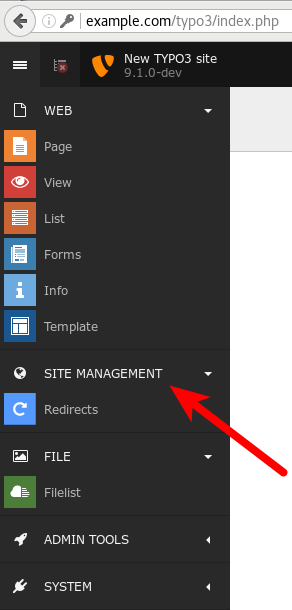
\includegraphics[width=0.45\linewidth]{BackendUserInterface/AddedNewMainModuleSiteManagement.png}
			\end{figure}
		\end{column}
		\begin{column}{.5\textwidth}
			Die neue Systemerweiterung \texttt{EXT:redirects} stellt die erste Komponente dieses
			Hauptmoduls dar (siehe nächste Seite für Details).
		\end{column}
		\begin{column}{.1\textwidth}
		\end{column}
	\end{columns}

\end{frame}

% ------------------------------------------------------------------------------
% LTXE-SLIDE-START
% LTXE-SLIDE-UID:		8bd6b85d-ed8c77e3-94a40b39-e15bb504
% LTXE-SLIDE-TITLE:		System Extension "Redirects" Has Been Added
% LTXE-SLIDE-REFERENCE:	Feature-83631-SystemExtensionRedirectsHasBeenAdded.rst
% ------------------------------------------------------------------------------

\begin{frame}[fragile]
	\frametitle{Backend User Interface}
	\framesubtitle{Weiterleitungen}

	Das neue Modul ermöglicht Integratoren und Editoren die Konfiguration von Weiterleitungen.
	Die Funktion enthält einen einfachen Hitcounter (muss aktiviert werden) und
	Weiterleitungen können unbegrenzt oder für einen bestimmten Zeitraum eingerichtet werden.

	\begin{figure}
		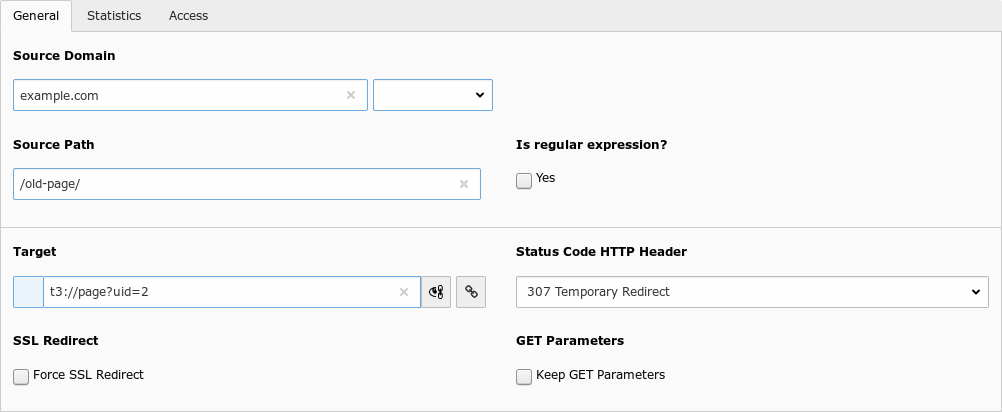
\includegraphics[width=0.8\linewidth]{BackendUserInterface/SystemExtensionRedirectsHasBeenAdded.png}
	\end{figure}

\end{frame}

% ------------------------------------------------------------------------------
% LTXE-SLIDE-START
% LTXE-SLIDE-UID:		e10a0f89-e91ecdb3-928841b6-1a84fc50
% LTXE-SLIDE-TITLE:		Show Fieldname Next To Title In Debug Mode
% LTXE-SLIDE-REFERENCE:	Feature-83461-ShowFieldnameNextToTitleInDebugMode.rst
% ------------------------------------------------------------------------------

\begin{frame}[fragile]
	\frametitle{Backend User Interface}
	\framesubtitle{Feldnamen im Debug-Modus}

	\begin{itemize}

		\item TYPO3 Integratoren und Entwickler beschäftigen sich oft mit Eingabefeldern im Backend,
			z.B. bei der Einrichtung von Berechtigungen oder während dem Schreiben von TsConfig.

		\item Anstatt in den Quellcode des Browsers zu schauen, werden Feldnamen für jedes Feld angezeigt,
			das von FormEngine generiert wird.

		\item Dies gilt nur für Benutzer mit Administratorrechten und erfordert
			dass der Denug-Modus in TYPO3 aktiviert wird.

			\smaller
				\texttt{\$GLOBALS['TYPO3\_CONF\_VARS']['BE']['debug']}
			\normalsize

	\end{itemize}

	\begin{figure}
		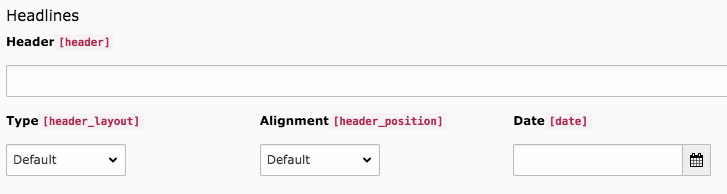
\includegraphics[width=0.60\linewidth]{BackendUserInterface/ShowFieldnameNextToTitleInDebugMode.png}
	\end{figure}

\end{frame}

% ------------------------------------------------------------------------------

% ------------------------------------------------------------------------------
% TYPO3 Version 9.3 - What's New - Chapter "Changes for Integrators" (German Version)
%
% @author	Michael Schams <schams.net>
% @license	Creative Commons BY-NC-SA 3.0
% @link		http://typo3.org/download/release-notes/whats-new/
% @language	German
% ------------------------------------------------------------------------------
% LTXE-CHAPTER-UID:		3a9852ea-e2360d9d-1ff5eec1-a7de3f9f
% LTXE-CHAPTER-NAME:	Changes for Integrators
% ------------------------------------------------------------------------------

\section{Änderungen für Integratoren}
\begin{frame}[fragile]
	\frametitle{Änderungen für Integratoren}

	\begin{center}\huge{Kapitel 2:}\end{center}
	\begin{center}\huge{\color{typo3darkgrey}\textbf{Änderungen für Integratoren}}\end{center}

\end{frame}

% ------------------------------------------------------------------------------
% LTXE-SLIDE-START
% LTXE-SLIDE-UID:		0e80eecb-f66842d4-e73c50c8-c2bb58a6
% LTXE-SLIDE-TITLE:		...
% LTXE-SLIDE-REFERENCE:	#84843 - Use no-cookie domain for youtube by default
% ------------------------------------------------------------------------------

\begin{frame}[fragile]
	\frametitle{Änderungen für Integratoren}
	\framesubtitle{No-Cookie-Domain für YouTube-Videos}

	% decrease font size for code listing
	\lstset{basicstyle=\smaller\ttfamily}

	\begin{itemize}
		\item Youtube-Videos werden standardmäßig über die No-Cookie-Domain
			\url{https://www.youtube-nocookie.com} gerendert
		\item Die reguläre Domain \texttt{www.youtube.com} kann bei Bedarf durch folgende
			TypoScript-Konfiguration erzwungen werden:

			\begin{lstlisting}
				lib.contentElement {
				  settings {
				    media {
				      additionalConfig {
				        no-cookie = 0
				      }
				    }
				  }
				}
			\end{lstlisting}

	\end{itemize}

\end{frame}

% ------------------------------------------------------------------------------
% LTXE-SLIDE-START
% LTXE-SLIDE-UID:		0e80eecb-f66842d4-e73c50c8-c2bb58a6
% LTXE-SLIDE-TITLE:		General Data Protection Regulation
% LTXE-SLIDE-REFERENCE:	#84843 - Use no-cookie domain for youtube by default
% LTXE-SLIDE-REFERENCE:	GDPR Initiative: https://forge.typo3.org/issues/84776
% ------------------------------------------------------------------------------

\begin{frame}[fragile]
	\frametitle{Änderungen für Integratoren}
	\framesubtitle{Datenschutz-Grundverordnung}

	\begin{itemize}
		\item  Um IP-Adressen mehrerer Datenbanktabellen nach bestimmter Zeit zu anonymisieren,
			kann der Scheduler-Task aktiviert werden.\newline

			Zum Beispiel die Tabelle \texttt{sys\_log}, nach 30 Tagen:
			\begin{figure}
				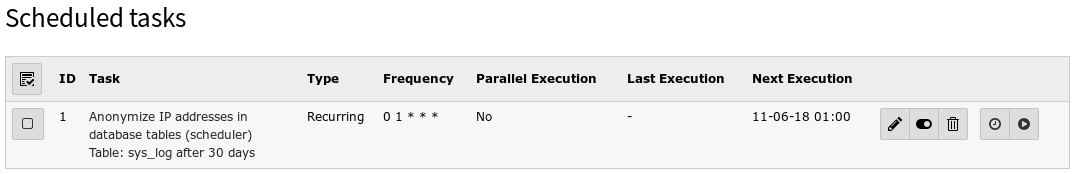
\includegraphics[width=1\linewidth]{ChangesForIntegrators/IpAnonymizationSchedulerTask.png}
			\end{figure}

		\item Der \href{https://typo3.com/blog/tag/gdpr/}{TYPO3 GmbH Blog}
			enthält weitere Informationen zur DSGVO
	\end{itemize}

\end{frame}

% ------------------------------------------------------------------------------
% LTXE-SLIDE-START
% LTXE-SLIDE-UID:		0e80eecb-f66842d4-e73c50c8-c2bb58a6
% LTXE-SLIDE-TITLE:		FE/BE User Accounts and Passwords
% LTXE-SLIDE-REFERENCE:	#85026 - salted passwords changes
% ------------------------------------------------------------------------------

\begin{frame}[fragile]
	\frametitle{Änderungen für Integratoren}
	\framesubtitle{FE/BE Benutzerkonten und Passwörter}

	% decrease font size for code listing
	\lstset{basicstyle=\tiny\ttfamily}

	\begin{itemize}
		\item Unverschlüsselte-Passwörter sind für BE/FE-Benutzer nicht mehr möglich
		\item Inaktive FE/BE Benutzerdatensätze können aus der Datenbank entfernt werden, indem der Schedular-Task
			"Table garbage collection task" hinzugefügt wird und "Clean all available tables"
			aktiviert wird\newline
			\smaller
				(Daten die nicht existieren können im Falle einer Sicherheitsverletzung nicht
				beeinträchtigt werden)
			\normalsize

			\begin{lstlisting}
				<?php
				$tableGarbageCollectionTask = \TYPO3\CMS\Scheduler\Task\TableGarbageCollectionTask::class;
				$GLOBALS['TYPO3_CONF_VARS']['SC_OPTIONS']['scheduler']['tasks'][$tableGarbageCollectionTask]
				  ['options']['tables'] = [
				  'be_users' => [
				    'dateField' => 'lastlogin',
				    'expirePeriod' => 30
				  ]
				];
			\end{lstlisting}

		\item Siehe \href{https://docs.typo3.org/typo3cms/extensions/scheduler/Installation/BaseTasks/Index.html}{die Dokumentation} für weitere Informationen
	\end{itemize}
\end{frame}

% ------------------------------------------------------------------------------
% LTXE-SLIDE-START
% LTXE-SLIDE-UID:		f38ee3cb-51d1aa0a-4f6884bf-adadc9e3
% LTXE-SLIDE-TITLE:		"Duplicate" Button
% LTXE-SLIDE-REFERENCE:	#84749 - Hide "duplicate" button by default
% ------------------------------------------------------------------------------

\begin{frame}[fragile]
	\frametitle{Änderungen für Integratoren}
	\framesubtitle{"Duplicate"-Taste}

	% decrease font size for code listing
	\lstset{basicstyle=\smaller\ttfamily}

	\begin{itemize}
		\item Die Taste zum duplizieren eines Inhaltelements ist jetzt standardmäßg ausgeblendet
		\item Die Sichtbarkeit kann durch TSconfig ("1" = enabled) aktiviert werden:

			\begin{lstlisting}
				options.showDuplicate = 1
				options.showDuplicate.[table] = 1
			\end{lstlisting}

	\end{itemize}
	\vspace{-0.5cm}
	\begin{figure}
		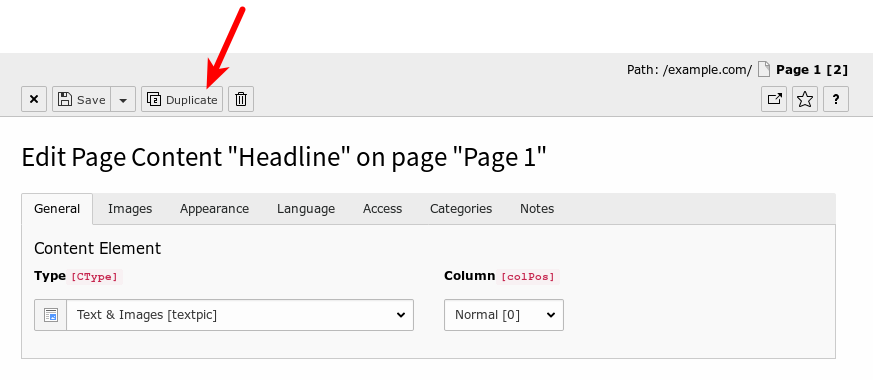
\includegraphics[width=0.8\linewidth]{ChangesForIntegrators/DuplicateButtonHiddenByDefault.png}
	\end{figure}

\end{frame}

% ------------------------------------------------------------------------------
% LTXE-SLIDE-START
% LTXE-SLIDE-UID:		0e80eecb-f66842d4-e73c50c8-c2bb58a6
% LTXE-SLIDE-TITLE:		HTML5 Date Form Element
% LTXE-SLIDE-REFERENCE:	#82511 - EXT:form add HTML5 date form element
% ------------------------------------------------------------------------------

\begin{frame}[fragile]
	\frametitle{Änderungen für Integratoren}
	\framesubtitle{\texttt{EXT:form} HTML5 Formularelement: Datum}

	% decrease font size for code listing
	\lstset{basicstyle=\tiny\ttfamily}

	\begin{itemize}
		\item Das Formularframework enthält ein neues Formularelement "\texttt{Date}",
			dazu gehört auch ein passender Validator
		\item Dies ist technisch ein HTML5 \texttt{'type=date'} Attribut
			(siehe \href{https://www.w3.org/TR/2011/WD-html-markup-20110405/input.date.html}{w3c.org})
		\item Ein Beispiel dafür (beinhaltet auch einen "DateRange" Validator):

			\begin{lstlisting}
				type: Date
				identifier: date-1
				label: Date
				defaultValue: '2018-03-02'
				properties:
				  displayFormat: 'd.m.Y'
				  fluidAdditionalAttributes:
				    min: '2018-03-01'
				    max: '2018-03-30'
				    step: '1'
				validators:
				  -
				    identifier: DateRange
				    options:
				      minimum: '2018-03-01'
				      maximum: '2018-03-30'
			\end{lstlisting}

	\end{itemize}

\end{frame}

% ------------------------------------------------------------------------------
% LTXE-SLIDE-START
% LTXE-SLIDE-UID:		0e80eecb-f66842d4-e73c50c8-c2bb58a6
% LTXE-SLIDE-TITLE:		Destructive Database Schema Changes
% LTXE-SLIDE-REFERENCE:	#85160 - Non destructive database schema changes in extension manager
% ------------------------------------------------------------------------------

\begin{frame}[fragile]
	\frametitle{Änderungen für Integratoren}
	\framesubtitle{Änderungen im Bezug auf destruktive Datenbankstruktur}

	\begin{itemize}
		\item Wenn eine Extension über den Extension-Manager installiert oder aktualisiert wird
			und \textit{destruktive} Datenbankänderungen erforderlich sind, werden diese Änderungen
			nicht automatisch angewendet
		\item "Destruktive" Änderungen sind zum Beispiel Änderungen von bestehenden Spalten, 
			Entfernen einer Spalte, Index- oder Tabellendefinition usw.
		\item Um diese besonderen Datenbank-Updates zu überprüfen und möglicherweise auszuführen
			gehen Sie bitte  in ADMIN TOOLS → Maintenance → Analyze Database Structure\newline
	\end{itemize}

	\vspace{-0.4cm}

	% Translators: remove the illustration below, if it does not fit on the
	% slide, e.g. in case your language requires more space. The illustration is
	% not really required, just "nice to have".

	\begin{figure}
		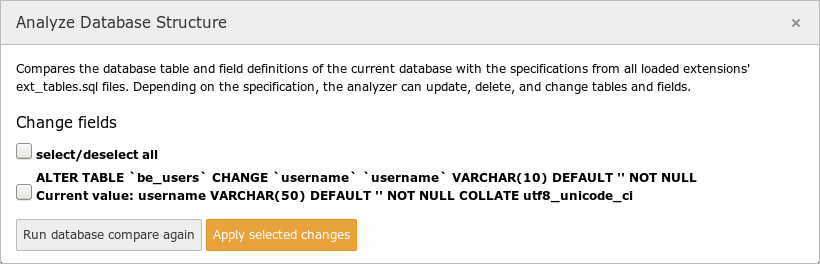
\includegraphics[width=0.6\linewidth]{ChangesForIntegrators/DestructiveDatabaseChanges.png}
	\end{figure}

\end{frame}

% ------------------------------------------------------------------------------
% LTXE-SLIDE-START
% LTXE-SLIDE-UID:		0e80eecb-f66842d4-e73c50c8-c2bb58a6
% LTXE-SLIDE-TITLE:		TypoScript Conditions
% LTXE-SLIDE-REFERENCE:	#84760 - TypoScript conditions for site and siteLanguage
% ------------------------------------------------------------------------------

\begin{frame}[fragile]
	\frametitle{Änderungen für Integratoren}
	\framesubtitle{TypoScript-Bedienungen}

	Neue TypoScript-Bedienung:

	\begin{itemize}
		\item Bedingung für die Eigenschaften eines Site-Objekts

			\begin{lstlisting}
				[site = identifier = someIdentifier, base = https://example.com/]
				  page.30.value = foo
				[global]
			\end{lstlisting}

		\item Bedingung für die Seitensprache

			\begin{lstlisting}
				[siteLanguage = locale = de_CH.UTF-8, title = Switzerland]
				  page.40.value = bar
				[global]
			\end{lstlisting}

	\end{itemize}

\end{frame}

% ------------------------------------------------------------------------------
% LTXE-SLIDE-START
% LTXE-SLIDE-UID:		0e80eecb-f66842d4-e73c50c8-c2bb58a6
% LTXE-SLIDE-TITLE:		HMENU cObj and language IDs
% LTXE-SLIDE-REFERENCE:	#84775 - Extend HMENU to support auto filling of special.value for special=language
% ------------------------------------------------------------------------------

\begin{frame}[fragile]
	\frametitle{Änderungen für Integratoren}
	\framesubtitle{\texttt{HMENU} cObj und Sprachen IDs}

	% decrease font size for code listing
	%\lstset{basicstyle=\tiny\ttfamily}

	\begin{itemize}
		\item \texttt{HMENU} Inhaltsobjekt unterstützt jetzt das automatische Ausfüllen von
			Sprach-IDs für Sprachmenüs

			\begin{lstlisting}
				10 = HMENU
				10 {
				  special = language
				  special.value = auto
				}
  			\end{lstlisting}

	\end{itemize}

\end{frame}

% ------------------------------------------------------------------------------
% LTXE-SLIDE-START
% LTXE-SLIDE-UID:		0e80eecb-f66842d4-e73c50c8-c2bb58a6
% LTXE-SLIDE-TITLE:		View User TSConfig Data
% LTXE-SLIDE-REFERENCE:	#85017 - User TSConfig shown in Configuration module
% ------------------------------------------------------------------------------

\begin{frame}[fragile]
	\frametitle{Änderungen für Integratoren}
	\framesubtitle{User TSconfig Daten anzeigen}

	User TSConfig Daten des aktuell angemeldeten Benutzers können unter  
	\textbf{System -> Configuration} gefunden werden

	\begin{figure}
		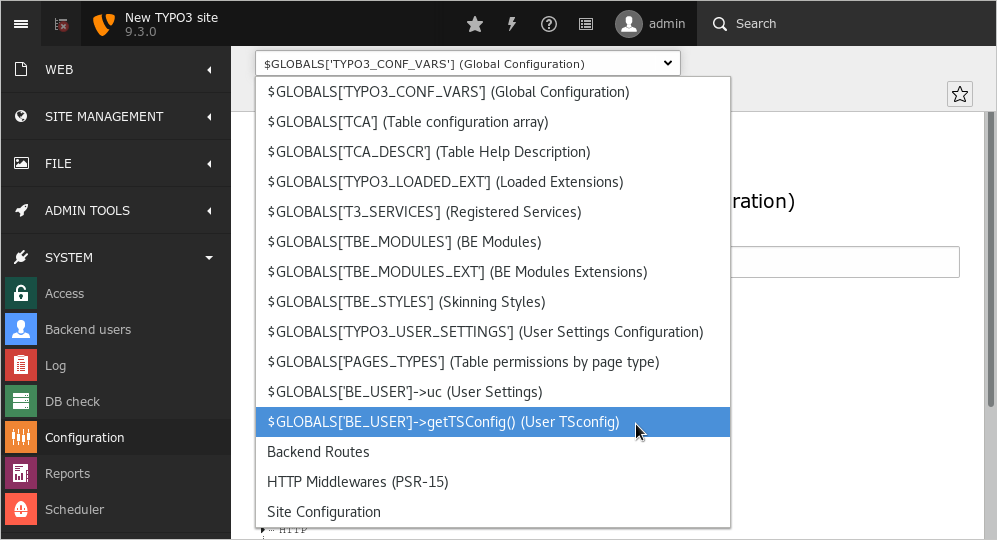
\includegraphics[width=0.75\linewidth]{ChangesForIntegrators/SystemConfigurationUserTSConfig.png}
	\end{figure}

\end{frame}

% ------------------------------------------------------------------------------
% LTXE-SLIDE-START
% LTXE-SLIDE-UID:		0e80eecb-f66842d4-e73c50c8-c2bb58a6
% LTXE-SLIDE-TITLE:		Miscellaneous
% LTXE-SLIDE-REFERENCE:	#69274 - Preserve image rotation if orient is saved in exif
% LTXE-SLIDE-REFERENCE:	#85147 - Render SEO meta tags in frontend
% LTXE-SLIDE-REFERENCE:	#84715 - Set exclude property for tt_content fields
% ------------------------------------------------------------------------------

\begin{frame}[fragile]
	\frametitle{Änderungen für Integratoren}
	\framesubtitle{Sonstiges}

	\begin{itemize}
		\item TYPO3 berücksichtigt beim Bearbeiten des Bildes (z.B. Skalierung/Zuschneiden
			die Bildausrichtung, die als EXIF-Angabe gespeichert wird
		\item SEO-bezogene Meta-Tags, die in den Seiteneigenschaften festgelegt sind,
			werden jetzt standardmäßg im Frontend gerendert
		\item Die \textit{exclude} Eigenschaft ist für folgende Felder festgelegt:

			\begin{itemize}
				\smaller
				\item \texttt{tt\_content.file\_collections}
				\item \texttt{tt\_content.filelink\_size}
				\item \texttt{tt\_content.filelink\_sorting}
				\item \texttt{tt\_content.filelink\_sorting\_direction}
			\end{itemize}

			\small
				Dalls Redakteure diese Felder bearbeiten dürfen, müssen die Zugriffberechtigungen 
				angepasst werden!
			\normalsize

	\end{itemize}

\end{frame}

% ------------------------------------------------------------------------------

% ------------------------------------------------------------------------------
% TYPO3 Version 9.2 - What's New - Chapter "Changes for Developers" (English Version)
%
% @author	Michael Schams <schams.net>
% @license	Creative Commons BY-NC-SA 3.0
% @link		http://typo3.org/download/release-notes/whats-new/
% @language	English
% ------------------------------------------------------------------------------
% LTXE-CHAPTER-UID:		846d40ce-66fdc2ec-750dcf95-33ce93e0
% LTXE-CHAPTER-NAME:	Changes for Developers
% ------------------------------------------------------------------------------

\section{Änderungen für Entwickler}
\begin{frame}[fragile]
	\frametitle{Änderungen für Entwickler}

	\begin{center}\huge{Kapitel 3:}\end{center}
	\begin{center}\huge{\color{typo3darkgrey}\textbf{Änderungen für Entwickler}}\end{center}

\end{frame}

% ------------------------------------------------------------------------------
% LTXE-SLIDE-START
% LTXE-SLIDE-UID:		c7b4f7f2-a11e6fc7-4ffe6e04-92cc98aa
% LTXE-SLIDE-TITLE:		PSR-15 Middlewares Support (1)
% LTXE-SLIDE-REFERENCE:	Feature-83725-SupportForPSR-15HTTPMiddlewares.html
% ------------------------------------------------------------------------------

\begin{frame}[fragile]
	\frametitle{Änderungen für Entwickler}
	\framesubtitle{PSR-15 Middlewares Unterstützung (1)}

	\begin{itemize}
		\item TYPO3 möchte den \href{https://www.php-fig.org/psr/psr-15/}{PSR-15 standard} out-of-the box
			unterstützen
		\item Dies wird die Interoperabilität mit unabhängigen Bibliotheken verbessern und alle 
			Anfragen im TYPO3-Kern werden eine PSR-7-Reaktion zurückgeben

		\item Die PSR-15 Standard wird folgenderweise definiert:
			\newline
			\smaller
				\textit{[PSR-15] describes common interfaces for HTTP server request handlers
				(request handlers) and HTTP server middleware components (middleware) that use
				HTTP messages [...]. HTTP request handlers are a fundamental part of any web
				application. Server side code receives a request message, processes it, and
				produces a response message. HTTP middleware is a way to move common request
				and response processing away from the application layer."}
				\newline
				Siehe \url{https://www.php-fig.org/psr/psr-15/} für weitere Informationen.
			\normalsize

	\end{itemize}

	% Note for translators: do not translate the PSR-15 definition above.
	% It is a quote from the php-fig.org website and should remain as it stands.

\end{frame}

% ------------------------------------------------------------------------------
% LTXE-SLIDE-START
% LTXE-SLIDE-UID:		c7b4f7f2-a11e6fc7-4ffe6e04-92cc98aa
% LTXE-SLIDE-TITLE:		PSR-15 Middlewares Support (2)
% LTXE-SLIDE-REFERENCE:	Feature-83725-SupportForPSR-15HTTPMiddlewares.html
% ------------------------------------------------------------------------------

\begin{frame}[fragile]
	\frametitle{Änderungen für Entwickler}
	\framesubtitle{PSR-15 Middlewares Unterstützung (2)}

	% decrease font size for code listing
	\lstset{basicstyle=\tiny\ttfamily}

	\begin{itemize}
		\item Um eine Middleware zu der "\textit{frontend}" oder "\textit{backend}"
			Middleware-Stack hinzuzufügen, muss eine \texttt{Configuration/RequestMiddlewares.php}
			Datei in der jeweiligen Extension erstellt werden:

			\begin{lstlisting}
				return [
				  // stack name: currently 'frontend' or 'backend'
				  'frontend' => [
				    'middleware-identifier' => [
				      'target' => \ACME\Ext\Middleware::class,
				      'description' => '',
				      'before' => [
				        'another-middleware-identifier',
				      ],
				      'after' => [
				        'yet-another-middleware-identifier',
				      ],
				    ]
				  ]
				];
			\end{lstlisting}

	\end{itemize}

\end{frame}

% ------------------------------------------------------------------------------
% LTXE-SLIDE-START
% LTXE-SLIDE-UID:		c7b4f7f2-a11e6fc7-4ffe6e04-92cc98aa
% LTXE-SLIDE-TITLE:		PSR-15 Middlewares Support (3)
% LTXE-SLIDE-REFERENCE:	Feature-83725-SupportForPSR-15HTTPMiddlewares.html
% ------------------------------------------------------------------------------

\begin{frame}[fragile]
	\frametitle{Änderungen für Entwickler}
	\framesubtitle{PSR-15 Middlewares Unterstützung (3)}

	% decrease font size for code listing
	\lstset{basicstyle=\tiny\ttfamily}

	\begin{itemize}

		\item Wenn Erweiterungen stillgelegt werden müssen oder vorhandene Middlewares durch eine eigene Lösung ersetzt werden 
			müssen, die vorhandene Middleware kann deaktiviert werden, indem man in der Datei
			folgenden Code hinzufügt:

			\begin{lstlisting}
				return [
				  'frontend' => [
				    'middleware-identifier' => [
				      'disabled' => true,
				    ],
				  ],
				];
			\end{lstlisting}

		\item Lesen Sie mehr über \href{https://new.typo3.org/community/teams/typo3-development/initiatives/initiative-psr-15/}{PSR-15 Initiative} 

	\end{itemize}

\end{frame}

% ------------------------------------------------------------------------------
% LTXE-SLIDE-START
% LTXE-SLIDE-UID:		c7b4f7f2-a11e6fc7-4ffe6e04-92cc98aa
% LTXE-SLIDE-TITLE:		Extended PSR-7 Requests with TYPO3 Normalized Server Parameters
% LTXE-SLIDE-REFERENCE:	Feature-83736-ExtendedPSR-7RequestsWithTYPO3ServerParameters
% ------------------------------------------------------------------------------

\begin{frame}[fragile]
	\frametitle{Änderungen für Entwickler}
	\framesubtitle{PSR-7 Serveranforderungen}

	% decrease font size for code listing
	\lstset{basicstyle=\tiny\ttfamily}

	\begin{itemize}

		\item PSR-7-basierte ServerRequest-Objekte enthalten ein TYPO3-spezifisches 
			Attributobjekt für normalisierte Serverparameter
		\item Das Objekt ist \textbf{momentan} als Attribut des 
			\texttt{ServerRequestInterface \$request} Objekte verfügbar.

			\begin{lstlisting}
				/** @var NormalizedParams $normalizedParams */
				$normalizedParams = $request->getAttribute('normalizedParams');
				$requestPort = $normalizedParams->getRequestPort();
			\end{lstlisting}

		\item Dies ersetzt \texttt{GeneralUtility::getIndpEnv()} und Behauptungen
			wie zum Beispiel \texttt{SCRIPT\_NAME}, \texttt{REQUEST\_URI}, usw können ersetzt werden
			\newline
			(siehe \href{https://docs.typo3.org/typo3cms/extensions/core/latest/Changelog/9.2/Feature-83736-ExtendedPSR-7RequestsWithTYPO3ServerParameters.html}{Dokumentation} für mehrere Informationen)

	\end{itemize}

\end{frame}

% ------------------------------------------------------------------------------
% LTXE-SLIDE-START
% LTXE-SLIDE-UID:		c7b4f7f2-a11e6fc7-4ffe6e04-92cc98aa
% LTXE-SLIDE-TITLE:		PSR-7 and PSR-15 Related Changes
% LTXE-SLIDE-REFERENCE:	Important-83724-APIAndBehaviorChangeInRequestHandlerClasses
% ------------------------------------------------------------------------------

\begin{frame}[fragile]
	\frametitle{Änderungen für Entwickler}
	\framesubtitle{Änderungen die zur PSR-7 and PSR-15 gehören}

	% decrease font size for code listing
	\lstset{basicstyle=\tiny\ttfamily}

	\begin{itemize}
		\item Die internen Request-Handler-Klassen wurden geändert:

		\begin{itemize}
			\item Alle Methoden haben strenge Argumente und Rückgabetypdeklarationen erhalten
			\item Anstatt \texttt{HttpUtility::redirect()},\newline
				ein \texttt{RedirectResponse} wird zurückgegeben
			\item Anstatt Null wird eine NullResponse zurückgegeben
		\end{itemize}

	\end{itemize}

\end{frame}

% ------------------------------------------------------------------------------
% LTXE-SLIDE-START
% LTXE-SLIDE-UID:		c7b4f7f2-a11e6fc7-4ffe6e04-92cc98aa
% LTXE-SLIDE-TITLE:		Environment Class
% LTXE-SLIDE-REFERENCE:	Feature-84153-IntroduceAGenericEnvironmentClass
% ------------------------------------------------------------------------------

\begin{frame}[fragile]
	\frametitle{Änderungen für Entwickler}
	\framesubtitle{Enwironment-Klasse}

	% decrease font size for code listing
	\lstset{basicstyle=\tiny\ttfamily}

	\begin{itemize}
		\item Die neue Basis-API-Klasse stellt anwendungsübergreifende Informationen zu Pfaden
			und PHP-internals, auf die bisher über PHP Konstanten zugegriffen werden konnte:
				\small
					\texttt{TYPO3\textbackslash
						CMS\textbackslash
						Core\textbackslash
						Core\textbackslash
						Environment}
				\normalsize

		\item Die folgenden statischen API-Methoden sind verfügbar:

			\begin{itemize}
				\smaller
				\item \texttt{Environment::isCli()}
					% defines whether TYPO3 runs on a CLI context or HTTP context
				\item \texttt{Environment::getApplicationContext()}
					% returns the ApplicationContext object that encapsulates TYPO3_CONTEXT
				\item \texttt{Environment::isComposerMode()}
					% defines whether TYPO3 was installed via composer
				\item \texttt{Environment::getProjectPath()}
					% returns the absolute path to the root-level folder without the trailing slash
				\item \texttt{Environment::getPublicPath()}
					% returns the absolute path to the publically accessible folder (previously known as PATH_site) without the trailing slash
				\item \texttt{Environment::getVarPath()}
					% returns the absolute path to the folder where non-public semi-persistent files can be stored. For regular projects, this is known as PATH_site/typo3temp/var
				\item \texttt{Environment::getConfigPath()}
					% returns the absolute path to the folder where (writeable) configuration is stored. For regular projects, this is known as PATH_site/typo3conf
				\item \texttt{Environment::getCurrentScript()}
					% the absolute path and filename to the currently executed PHP script
				\item \texttt{Environment::isWindows()}
					% whether TYPO3 runs on a windows server
				\item \texttt{Environment::isUnix()}
					% whether TYPO3 runs on a unix server
			\end{itemize}

	\end{itemize}

\end{frame}

% ------------------------------------------------------------------------------
% LTXE-SLIDE-START
% LTXE-SLIDE-UID:		c7b4f7f2-a11e6fc7-4ffe6e04-92cc98aa
% LTXE-SLIDE-TITLE:		Add recursive filtering of arrays
% LTXE-SLIDE-REFERENCE:	83350-AddRecursiveArrayFiltering
% ------------------------------------------------------------------------------

\begin{frame}[fragile]
	\frametitle{Änderungen für Entwickler}
	\framesubtitle{String Constraints suchen}

	% decrease font size for code listing
	\lstset{basicstyle=\tiny\ttfamily}

	\begin{itemize}
		\item Ein neuer Hook ermöglicht die Änderung von Suchtechnischen Einschränkungen:

			\begin{lstlisting}
				// EXT:my_site/ext_localconf.php
				$dbRecordList = \TYPO3\CMS\Recordlist\RecordList\DatabaseRecordList::class;
				$GLOBALS['TYPO3_CONF_VARS']['SC_OPTIONS'][$dbRecordList]['makeSearchStringConstraints'][123] =
				  \MyVendor\MySite\Hooks\DatabaseRecordListHook::class . '->makeSearchStringConstraints';
			\end{lstlisting}

			\begin{lstlisting}
				// EXT:my_site/Classes/Hooks/DatabaseRecordListHook.php
				namespace MyVendor\MySite\Hooks;
				class DatabaseRecordListHook
				{
				  public function makeSearchStringConstraints(
				    \TYPO3\CMS\Core\Database\Query\QueryBuilder $queryBuilder
				    array $constraints,
				    string $searchString,
				    string $table,
				    int $currentPid,
				  ) {
				    return $constraints;
				  }
				}
			\end{lstlisting}

	\end{itemize}

\end{frame}

% ------------------------------------------------------------------------------
% LTXE-SLIDE-START
% LTXE-SLIDE-UID:		c7b4f7f2-a11e6fc7-4ffe6e04-92cc98aa
% LTXE-SLIDE-TITLE:		Signal/Slot for User Switch
% LTXE-SLIDE-REFERENCE:	Feature-80263-AddANewSignalSlotForUserSwitch
% ------------------------------------------------------------------------------

\begin{frame}[fragile]
	\frametitle{Änderungen für Entwickler}
	\framesubtitle{Signal/Slot für User Switch}

	% decrease font size for code listing
	\lstset{basicstyle=\tiny\ttfamily}

	\begin{itemize}
		\item Ein neues Signal wird ausgegeben, wenn ein Admin-Benutzer im TYPO3-Backend zu einem
			anderen Benutzer wechselt

			\begin{lstlisting}
				$dispatcher = \TYPO3\CMS\Core\Utility\GeneralUtility::makeInstance(
				  \TYPO3\CMS\Extbase\SignalSlot\Dispatcher::class
				);

				$dispatcher->connect(
				  \TYPO3\CMS\Beuser\Controller\BackendUserController::class,
				  'switchUser',
				  \MyVendor\MyExtension\Slots\BackendUserController::class,
				  'switchUser'
				);
			\end{lstlisting}

	\end{itemize}

\end{frame}

% ------------------------------------------------------------------------------
% LTXE-SLIDE-START
% LTXE-SLIDE-UID:		c7b4f7f2-a11e6fc7-4ffe6e04-92cc98aa
% LTXE-SLIDE-TITLE:		ViewHelper Changes (1)
% LTXE-SLIDE-REFERENCE:	Feature-82704-AddReadonlyAndRequiredAttributesToTextareaViewHelper
% ------------------------------------------------------------------------------

\begin{frame}[fragile]
	\frametitle{Änderungen für Entwickler}
	\framesubtitle{ViewHelper Änderungen (1)}

	% decrease font size for code listing
	\lstset{basicstyle=\tiny\ttfamily}

	\begin{itemize}
		\item ViewHelper \texttt{f:form.textarea} unterstützt zwei neue Attribute\newline
			 "\texttt{readonly}" and "\texttt{required}"

			\begin{lstlisting}
				<!-- Set required attribute -->
				<f:form.textarea name="foobar" required="1" />

				<!-- Set readonly attribute -->
				<f:form.textarea name="foobar" readonly="1" />
			\end{lstlisting}

		\item ViewHelpers \texttt{f:uri.typolink} und \texttt{f:uri.typolink} unterstützen das neue
			Attribut "\texttt{absolute}"

			\begin{lstlisting}
				<f:link.typolink parameter="23" absolute="true">Link</f:link.typolink>
				<f:uri.typolink parameter="23" absolute="true" />
			\end{lstlisting}

		\item ViewHelper \texttt{f:render} unterstützt das neue Attribut "\texttt{debug}"
			das ermöglicht die Debug-Ausgabe in einigen Spezielfällen zu deaktivieren

	\end{itemize}

\end{frame}

% ------------------------------------------------------------------------------
% LTXE-SLIDE-START
% LTXE-SLIDE-UID:		c7b4f7f2-a11e6fc7-4ffe6e04-92cc98aa
% LTXE-SLIDE-TITLE:		ViewHelper Changes (2)
% LTXE-SLIDE-REFERENCE:	Feature-83942-ProvideViewHelperToRenderIconForResources
% ------------------------------------------------------------------------------

\begin{frame}[fragile]
	\frametitle{Änderungen für Entwickler}
	\framesubtitle{ViewHelper Änderungen (2)}

	% decrease font size for code listing
	\lstset{basicstyle=\tiny\ttfamily}

	\begin{itemize}
		\item Der neue ViewHelper gibt das Icon-Markup wieder basierend auf einer FAL-Resource

%			\begin{lstlisting}
%				<core:iconForResource resource="{file}" />
%			\end{lstlisting}

			\smaller
				\texttt{<core:iconForResource resource="\{file\}" />}
			\normalsize

	\end{itemize}

\end{frame}

% ------------------------------------------------------------------------------
% LTXE-SLIDE-START
% LTXE-SLIDE-UID:		c7b4f7f2-a11e6fc7-4ffe6e04-92cc98aa
% LTXE-SLIDE-TITLE:		Admin Panel Customization
% LTXE-SLIDE-REFERENCE:	Feature-84045-NewAdminPanelModuleAPI
% ------------------------------------------------------------------------------

\begin{frame}[fragile,label=AdminPanelCustomization]
	\frametitle{Änderungen für Entwickler}
	\framesubtitle{Admin Panel Anpassung}

	% decrease font size for code listing
	\lstset{basicstyle=\tiny\ttfamily}

	\begin{itemize}
		\item Das Admin Panel kann durch benutzerdefinierte Module erweitert werden:
		\item Modulregistrierungsbeispiel:

			\begin{lstlisting}
				$GLOBALS['TYPO3_CONF_VARS']['EXTCONF']['adminpanel']['modules']['yourmodulename'] = [
				  'module' => \MyVendor\Package\AdminPanel\YourModule::class,
				  'after' => ['preview']
				]
			\end{lstlisting}

	\end{itemize}

\end{frame}

% ------------------------------------------------------------------------------

% ------------------------------------------------------------------------------
% TYPO3 Version 9.4 - What's New (German Version)
%
% @license	Creative Commons BY-NC-SA 3.0
% @link		https://typo3.org/help/documentation/whats-new/
% @language	German
% ------------------------------------------------------------------------------

\section{Veraltete/Entfernte Funktionen}
\begin{frame}[fragile]
	\frametitle{Veraltete/Entfernte Funktionen}

	\begin{center}\huge{Kapitel 4:}\end{center}
	\begin{center}\huge{\color{typo3darkgrey}\textbf{Veraltete/Entfernte Funktionen}\end{center}

\end{frame}

% ------------------------------------------------------------------------------
% #65578 - Deprecate enableConcatenateFiles
% #84414 - BackendUtility::shortcutExists
% #85858 - Deprecate GeneralUtility::clientInfo()
% #85699 - Deprecate methods in PageRepository
% #85759 - Deprecate GeneralUtility::getHostName
% #85760 - Deprecate GeneralUtility::unQuoteFilenames
% #85394 - Deprecate TYPO3\CMS\Core\Database\PdoHelper

\begin{frame}[fragile]
	\frametitle{Veraltete/Entfernte Funktionen}
	\framesubtitle{Veraltete Optionen und Funktionen (1)}

	\begin{itemize}
		\item Die folgenden zwei TypoScript-Optionen wurden als veraltet markiert:

			\begin{itemize}\smaller
                \item \texttt{config.enableConcatenateFiles}
                \item \texttt{config.concatenateJsAndCss}
            \end{itemize}

        	\smaller
				Der letzterer wurde durch \texttt{concatenateCss} bzw
					\texttt{concatenateJs} ersetzt
			\normalsize

		\item Die folgenden Methoden / Klassen wurden als veraltet markiert:

			\begin{itemize}\smaller
				\item \texttt{TYPO3\textbackslash
					CMS\textbackslash
					Backend\textbackslash
					Utility\textbackslash
					BackendUtility::shortcutExists()}

				\item \texttt{TYPO3\textbackslash
					CMS\textbackslash
					Core\textbackslash
					Utility\textbackslash
					GeneralUtility::clientInfo()}

				\item \texttt{TYPO3\textbackslash
					CMS\textbackslash
					Core\textbackslash
					Utility\textbackslash
					GeneralUtility::getHostName()}

				\item \texttt{TYPO3\textbackslash
					CMS\textbackslash
					Core\textbackslash
					Utility\textbackslash
					GeneralUtility::unQuoteFilenames()}

				\item \texttt{TYPO3\textbackslash
					CMS\textbackslash
					Frontend\textbackslash
					Page\textbackslash
					PageRepository::getRecordsByField()}

				\item \texttt{TYPO3\textbackslash
					CMS\textbackslash
					Frontend\textbackslash
					Page\textbackslash
					PageRepository::getFileReferences()}

				\item \texttt{TYPO3\textbackslash
					CMS\textbackslash
					Core\textbackslash
					Database\textbackslash
					PdoHelper}

			\end{itemize}
	\end{itemize}

\end{frame}

% ------------------------------------------------------------------------------
% #85701 - Deprecate methods in ModuleTemplate
% #85707 - Deprecate LoginFramesetController

\begin{frame}[fragile]
	\frametitle{Veraltete/Entfernte Funktionen}
	\framesubtitle{Veraltete Optionen und Funktionen (2)}

	\begin{itemize}
		\item Die folgenden Methoden / Klassen wurden als veraltet markiert:

			\begin{itemize}\smaller
				\item \texttt{TYPO3\textbackslash
					CMS\textbackslash
					Backend\textbackslash
					Template\textbackslash
					ModuleTemplate::icons()}

				\item \texttt{TYPO3\textbackslash
					CMS\textbackslash
					Backend\textbackslash
					Template\textbackslash
					ModuleTemplate::loadJavascriptLib()}

			\end{itemize}

		\item Folgende Klasse wurde als veraltet markiert und die Funktionalität der Klasse wurde durch eine
			Anfrage an \texttt{index.php?loginRefresh=1} ersetzt:
			
			\begin{itemize}\smaller
				\item \texttt{TYPO3\textbackslash
					CMS\textbackslash
					Backend\textbackslash
					Controller\textbackslash
					LoginFramesetController}
			\end{itemize}\smaller

	\end{itemize}

\end{frame}

% ------------------------------------------------------------------------------
% #85793 - Deprecate several constants from SystemEnvironmentBuilder

\begin{frame}[fragile]
	\frametitle{Veraltete/Entfernte Funktionen}
	\framesubtitle{Veraltete Konstanten (1)}

	\begin{itemize}
		\item Folgende Konstanten sind veraltet (1/2)\newline
			und sollten nicht mehr verwendet werden:

			\begin{itemize}\smaller
				\item \texttt{TYPO3\_URL\_MAILINGLISTS}
				\item \texttt{TYPO3\_URL\_DOCUMENTATION}
				\item \texttt{TYPO3\_URL\_DOCUMENTATION\_TSREF}
				\item \texttt{TYPO3\_URL\_DOCUMENTATION\_TSCONFIG}
				\item \texttt{TYPO3\_URL\_CONSULTANCY}
				\item \texttt{TYPO3\_URL\_CONTRIBUTE}
				\item \texttt{TYPO3\_URL\_SECURITY}
				\item \texttt{TYPO3\_URL\_DOWNLOAD}
				\item \texttt{TYPO3\_URL\_SYSTEMREQUIREMENTS}
			\end{itemize}

	\end{itemize}

\end{frame}

% ------------------------------------------------------------------------------
% #85793 - Deprecate several constants from SystemEnvironmentBuilder
% #85285 - Replace last occurrences of PATH_site with Environment API

\begin{frame}[fragile]
	\frametitle{Veraltete/Entfernte Funktionen}
	\framesubtitle{Veraltete Konstanten (2)}

	\begin{itemize}
		\item Folgende Konstanten sind veraltet(2/2)\newline
			und sollten nicht mehr verwendet werden:

			\begin{itemize}\smaller
				\item \texttt{NUL}\tabto{3cm}(use \texttt{"\textbackslash 0"} instead)
				\item \texttt{TAB}\tabto{3cm}(use \texttt{"\textbackslash t"} instead)
				\item \texttt{SUB}\tabto{3cm}(use \texttt{chr(26)} instead)
				\item \texttt{PATH\_thisScript}\tabto{3cm}(use \texttt{Environment::getCurrentScript()} instead)
				\item \texttt{PATH\_site}\tabto{3cm}(use \texttt{Environment::getPublicPath().'/'} instead)
			\end{itemize}
	\end{itemize}

\end{frame}

% ------------------------------------------------------------------------------
% #85878 - Deprecate EidUtility and methods within TSFE

\begin{frame}[fragile]
	\frametitle{Veraltete/Entfernte Funktionen}
	\framesubtitle{\texttt{EidUtility} Klasse und \texttt{TSFE} Methoden}

	% decrease font size for code listing
	\lstset{basicstyle=\tiny\ttfamily}

	\begin{itemize}
		\item Folgende Klasse wurde als veraltet markiert:\newline
			\smaller\texttt{TYPO3\textbackslash
				CMS\textbackslash
				Frontend\textbackslash
				Utility\textbackslash
				EidUtility}\normalsize

		\item Folgende Methoden wurden als veraltet markiert:\newline
			\smaller\texttt{TYPO3\textbackslash
				CMS\textbackslash
				Frontend\textbackslash
				Controller\textbackslash
				TypoScriptFrontendController}\normalsize

				\begin{itemize}\smaller
					\item \texttt{TypoScriptFrontendController::initFEuser()}
					\item \texttt{TypoScriptFrontendController::storeSessionData()}
					\item \texttt{TypoScriptFrontendController::previewInfo()}
					\item \texttt{TypoScriptFrontendController::hook\_eofe()}
					\item \texttt{TypoScriptFrontendController::addTempContentHttpHeaders()}
					\item \texttt{TypoScriptFrontendController::sendCacheHeaders()}
				\end{itemize}

			\item Folgender Hook wurde als veraltet markiert:

				\begin{lstlisting}
$GLOBALS['TYPO3_CONF_VARS']['SC_OPTIONS']['tslib/class.tslib_fe.php']['hook_previewInfo']
				\end{lstlisting}

	\end{itemize}

\end{frame}

% ------------------------------------------------------------------------------
% #85004 - Deprecate methods in ReflectionService

\begin{frame}[fragile]
	\frametitle{Veraltete/Entfernte Funktionen}
	\framesubtitle{Die Klasse \texttt{ReflectionService}}

	\begin{itemize}
		\item Folgende Methoden wurden als veraltet markiert:\newline
			\smaller\texttt{TYPO3\textbackslash
				CMS\textbackslash
				Extbase\textbackslash
				Reflection\textbackslash
				ReflectionService}\normalsize

				\begin{itemize}\smaller
					\item \texttt{ReflectionService::getClassTagsValues()}
					\item \texttt{ReflectionService::getClassTagValues()}
					\item \texttt{ReflectionService::getClassPropertyNames()}
					\item \texttt{ReflectionService::hasMethod()}
					\item \texttt{ReflectionService::getMethodTagsValues()}
					\item \texttt{ReflectionService::getMethodParameters()}
					\item \texttt{ReflectionService::getPropertyTagsValues()}
					\item \texttt{ReflectionService::getPropertyTagValues()}
					\item \texttt{ReflectionService::isClassTaggedWith()}
					\item \texttt{ReflectionService::isPropertyTaggedWith()}
				\end{itemize}

	\end{itemize}

\end{frame}

% ------------------------------------------------------------------------------
% More functions have been deprecated/removed...

\begin{frame}[fragile]
	\frametitle{Veraltete/Entfernte Funktionen}

	\vspace{0.6cm}
	\begin{center}
		Viele weitere Funktionen
	\end{center}
	\vspace{-0.8cm}
	\begin{center}
		wurden in der TYPO3 Version 9.4
	\end{center}
	\vspace{-0.8cm}
	\begin{center}
		als veraltet markiert oder entfernt.
	\end{center}
	\vspace{-0.6cm}
	\begin{center}
		Bitte die
\href{https://docs.typo3.org/typo3cms/extensions/core/latest/Changelog/9.4/Index.html#deprecation}{TYPO3 Dokumentation} prüfen für weitere Informationen.
	\end{center}

\end{frame}

% ------------------------------------------------------------------------------

% ------------------------------------------------------------------------------
% TYPO3 Version 9.1 - What's New - Chapter "Miscellaneous" (English Version)
%
% @author	Michael Schams <schams.net>
% @license	Creative Commons BY-NC-SA 3.0
% @link		http://typo3.org/download/release-notes/whats-new/
% @language	English
% ------------------------------------------------------------------------------
% LTXE-CHAPTER-UID:		68197358-0dc32ac8-dea3141e-8267c2d8
% LTXE-CHAPTER-NAME:	Miscellaneous
% ------------------------------------------------------------------------------

\section{Sonstiges}
\begin{frame}[fragile]
	\frametitle{Sonstiges}

	\begin{center}\huge{Kapitel 5:}\end{center}
	\begin{center}\huge{\color{typo3darkgrey}\textbf{Sonstiges}}\end{center}

\end{frame}

% ------------------------------------------------------------------------------
% LTXE-SLIDE-START
% LTXE-SLIDE-UID:		83881e38-1600f572-38226367-85056be9
% LTXE-SLIDE-TITLE:		Upgrade Libraries
% LTXE-SLIDE-REFERENCE:	https://forge.typo3.org/issues/83490
% ------------------------------------------------------------------------------

\begin{frame}[fragile]
	\frametitle{Sonstiges}
	\framesubtitle{Aktualisierte Bibliotheken}

	\begin{itemize}
		\item "doctrine/dbal" wurde auf Version 2.6.3 aktualisiert\newline
			\smaller
				\href{http://doctrine-project.org}{http://doctrine-project.org}
			\normalsize

		\item "CKEditor" wurde auf Version 4.8.0 aktualisiert\newline
 			\smaller
				\href{https://ckeditor.com}{https://ckeditor.com}
			\normalsize

		\item "D3.js" wurde auf Version 4.12.2 aktualisiert\newline
			\smaller
				\href{https://d3js.org}{https://d3js.org}
			\normalsize

		\item "Moment.js" wurde auf Version 2.20.1 aktualisiert\newline
			\smaller
				\href{https://momentjs.com}{https://momentjs.com}
			\normalsize

		\item "CodeMirror" wurde auf Version 5.33.0 aktualisiert\newline
			\smaller
				\href{https://codemirror.net}{https://codemirror.net}
			\normalsize

		\item "imagesLoaded" wurde auf Version 4.1.4 aktualisiert\newline
			\smaller
				\href{https://imagesloaded.desandro.com}{https://imagesloaded.desandro.com}
			\normalsize

	\end{itemize}

\end{frame}

% ------------------------------------------------------------------------------

% ------------------------------------------------------------------------------
% TYPO3 Version 9.1 - What's New - Chapter "Sources" (English Version)
%
% @author	Michael Schams <schams.net>
% @license	Creative Commons BY-NC-SA 3.0
% @link		http://typo3.org/download/release-notes/whats-new/
% @language	English
% ------------------------------------------------------------------------------
% LTXE-CHAPTER-UID:		b28441c6-44c982a3-35fcefd3-f4dc5d5c
% LTXE-CHAPTER-NAME:	Sources and Authors
% ------------------------------------------------------------------------------

\section{Quellen und Autoren}
\begin{frame}[fragile]
	\frametitle{Quellen und Autoren}

	\begin{center}\huge{Kapitel 6:}\end{center}
	\begin{center}\huge{\color{typo3darkgrey}\textbf{Quellen und Autoren}}\end{center}

\end{frame}

% ------------------------------------------------------------------------------
% LTXE-SLIDE-START
% LTXE-SLIDE-UID:		51b2cb0b-b390885b-49e40a7d-63be1365
% LTXE-SLIDE-TITLE:		Sources
% ------------------------------------------------------------------------------

\begin{frame}[fragile]
	\frametitle{Quellen und Autoren}
	\framesubtitle{Quellen}

	\textbf{TYPO3 News:}
		\begin{itemize}\smaller
			\item \url{https://typo3.org/news}
		\end{itemize}

	\textbf{Release Infos:}
		\begin{itemize}\smaller
			\item \url{https://get.typo3.org/release-notes/9.x/TYPO3_CMS_9.1.0}
			\item \href{https://github.com/TYPO3/TYPO3.CMS/blob/master/INSTALL.md}{INSTALL.md}
				und \href{https://github.com/TYPO3/TYPO3.CMS/tree/master/typo3/sysext/core/Documentation/Changelog}{ChangeLog}
			\item \texttt{typo3/sysext/core/Documentation/Changelog/9.1/*}
		\end{itemize}

	\textbf{TYPO3 Bug-/Issuetracker:}
		\begin{itemize}\smaller
			\item \url{https://forge.typo3.org/projects/typo3cms-core}
		\end{itemize}

	\textbf{TYPO3 und Fluid Git Repositories:}
		\begin{itemize}\smaller
			\item \url{https://git.typo3.org/Packages/TYPO3.CMS.git}
			\item \url{https://github.com/TYPO3/Fluid}
		\end{itemize}

\end{frame}

% ------------------------------------------------------------------------------
% LTXE-SLIDE-START
% LTXE-SLIDE-UID:		98970217-deba22a1-cd6ec09f-b8d5e671
% LTXE-SLIDE-TITLE:		Authors
% ------------------------------------------------------------------------------

\begin{frame}[fragile]
	\frametitle{Quellen und Autoren}

	\vspace{-0.6cm}

	\centerline{\textbf{TYPO3 CMS What's New Team:}}

	\begin{center}
		\centerline{Pierrick Caillon, Richard Haeser, Jigal van Hemert}
		\centerline{Henrietta Kucsovan, Michael Schams and Roberto Torresani}
	\end{center}

	\vspace{0.8cm}

	\smaller\begin{center}\url{https://typo3.org/download/release-notes/whats-new}\end{center}\normalsize

	\vspace{1cm}

	\smaller\begin{center}Licensed under Creative Commons BY-NC-SA 3.0\end{center}\normalsize
	\begin{figure}\vspace*{-0.4cm}
		
\includegraphics[width=1.4cm]{SourcesAndAuthors/CreativeCommons-BY-NC-SA.png}
	\end{figure}

\end{frame}

% ------------------------------------------------------------------------------


% ------------------------------------------------------------------------------

%% ------------------------------------------------------------------------------
% TYPO3 - What's New - Test/Example Chapter
%
% @license	Creative Commons BY-NC-SA 3.0
% @link		https://typo3.org/help/documentation/whats-new/
% @language	Italian
% ------------------------------------------------------------------------------
% Test/Example Chapter
% ------------------------------------------------------------------------------

\section{Test Chapter}
\begin{frame}[fragile]
	\frametitle{Test Chapter}

	\begin{center}\huge{Test Chapter:}\end{center}
	\begin{center}\huge{\color{typo3darkgrey}\textbf{LaTeX Styles, Formatting, etc.}}\end{center}

\end{frame}

% ------------------------------------------------------------------------------
% Example: Font Styles (Formatting)
% ------------------------------------------------------------------------------

\begin{frame}
	\frametitle{Test Chapter}
	\framesubtitle{Font Styles}

	\begin{itemize}
		\item \emph{emphasis}
		\item \textsf{Sans}
		\item \texttt{teletypefont}
		\item \textit{italic}
		\item \underline{underline}
		\item \uppercase{uppercase}
		\item \textbf{bold}
		\item \alert{alert}
		\item
			\begingroup
				\color{typo3orange}
				typo3orange
			\endgroup

	\end{itemize}

\end{frame}

% ------------------------------------------------------------------------------
% Example: Links And Levels
% ------------------------------------------------------------------------------

\begin{frame}
	\frametitle{Test Chapter}
	\framesubtitle{Links}

	\begin{itemize}
		\item Item
		\item Item with link: \url{https://example.com}
		\item Item with \href{https://example.com}{link label}

		\item First level
		\begin{itemize}
			\item Second level
			\begin{itemize}
				\item Third level
			\end{itemize}
		\end{itemize}

	\end{itemize}

\end{frame}

% ------------------------------------------------------------------------------
% Example: Item List
% ------------------------------------------------------------------------------

\begin{frame}
	\frametitle{Test Chapter}
	\framesubtitle{Item List}

	\begin{itemize}
		\item Item 1
		\item Item 2
		\item Item 3
		\item Item 4
		\item Item 5
		\item Item 6
		\item Item 7
		\item Item 8
		\item Item 9
		\item Item 10
		\item Item 11
		\item Item 12
	\end{itemize}

\end{frame}

% ------------------------------------------------------------------------------
% Example: Two Columns
% ------------------------------------------------------------------------------

\begin{frame}
	\frametitle{Test Chapter}
	\framesubtitle{Two Columns}

	\begin{columns}[T]

		\begin{column}{.5\textwidth}
			\begin{itemize}
				\item Item 1
				\item Item 2
				\item Item 3
				\item Item 4
				\item Item 5
				\item Item 6
			\end{itemize}
		\end{column}

		\begin{column}{.5\textwidth}
			\begin{itemize}
				\item Item 7
				\item Item 8
				\item Item 9
				\item Item 10
				\item Item 11
				\item Item 12
			\end{itemize}
		\end{column}

	\end{columns}

\end{frame}

% ------------------------------------------------------------------------------
% Example: Code Snippet
% ------------------------------------------------------------------------------

\begin{frame}[fragile]
	\frametitle{Test Chapter}
	\framesubtitle{Code Snippets}

	\begin{itemize}
		\item code outside a bullet list:
	\end{itemize}

	\begin{lstlisting}
		page = PAGE
		page.10 = TEXT
		page.10.value = Hello World
	\end{lstlisting}

	\begin{itemize}
		\item code inside a bullet list (indented):
		\begin{lstlisting}
			page = PAGE
			page.10 = TEXT
			page.10.value = Hello World
		\end{lstlisting}
	\end{itemize}

	\begin{itemize}
		\item inline code: \lstinline!var i:integer;!
		\item inline code: \texttt{var i:integer}
	\end{itemize}

\end{frame}

% ------------------------------------------------------------------------------
% Example: Code Snippet
% ------------------------------------------------------------------------------

\begin{frame}[fragile]
	\frametitle{Test Chapter}
	\framesubtitle{Code Snippets}

	\begin{itemize}
		\item custom font sizes (if not avoidable):

		\lstset{
			basicstyle=\large\selectfont\ttfamily
		}

		\begin{lstlisting}
			page = PAGE
			page.10 = TEXT
			page.10.value = Hello World
		\end{lstlisting}

		\lstset{
			basicstyle=\small\selectfont\ttfamily
		}

		\begin{lstlisting}
			page = PAGE
			page.10 = TEXT
			page.10.value = Hello World
		\end{lstlisting}

		\lstset{
			basicstyle=\fontsize{7}{9}\selectfont\ttfamily
		}

		\begin{lstlisting}
			page = PAGE
			page.10 = TEXT
			page.10.value = Hello World
		\end{lstlisting}

		\lstset{
			basicstyle=\tiny\ttfamily
		}

		\begin{lstlisting}
			page = PAGE
			page.10 = TEXT
			page.10.value = Hello World
		\end{lstlisting}

	\end{itemize}

%	\tabto{1cm} \texttt{custom indentation: 1cm from left}\newline
%	\tabto{1.5cm} \texttt{custom indentation: 1.5cm from left}\newline
%	\tabto{2cm} \texttt{custom indentation: 2cm from left}\newline
%	\tabto{2.5cm} \texttt{custom indentation: 2.5cm from left}\newline

\end{frame}

% ------------------------------------------------------------------------------
% Example: Slide Without Bullet Points
% ------------------------------------------------------------------------------

\begin{frame}
	\frametitle{Test Chapter}
	\framesubtitle{A Slide Without Bullet Points}

	Lorem ipsum dolor sit amet, consectetur adipisicing elit, sed do eiusmod
	tempor incididunt ut labore et dolore magna aliqua. Ut enim ad minim veniam,
	quis nostrud exercitation ullamco laboris nisi ut aliquip ex ea commodo
	consequat. Duis aute irure dolor in reprehenderit in voluptate velit esse
	cillum dolore eu fugiat nulla pariatur. Excepteur sint occaecat cupidatat
	non proident, sunt in culpa qui officia deserunt mollit anim id est laborum.

	%\breakingchange{BREAKING CHANGE!}
	\breakingchange

\end{frame}

% ------------------------------------------------------------------------------
% Example: Text Sizes
% ------------------------------------------------------------------------------

\begin{frame}
	\frametitle{Test Chapter}
	\framesubtitle{Text Sizes}

	\begin{itemize}
		\item Default text size ("normalsize"):\newline
			Lorem ipsum dolor sit amet, consectetur adipisicing elit, sed do eiusmod tempor incididunt ut labore et dolore magna aliqua.

		\item Small text size:\newline
			\small
				Lorem ipsum dolor sit amet, consectetur adipisicing elit, sed do eiusmod tempor incididunt ut labore et dolore magna aliqua.
			\normalsize

		\item Smaller text size:\newline
			\smaller
				Lorem ipsum dolor sit amet, consectetur adipisicing elit, sed do eiusmod tempor incididunt ut labore et dolore magna aliqua.
			\normalsize

		\item Tiny text size:\newline
			\tiny
				Lorem ipsum dolor sit amet, consectetur adipisicing elit, sed do eiusmod tempor incididunt ut labore et dolore magna aliqua.
			\normalsize

	\end{itemize}
\end{frame}

% ------------------------------------------------------------------------------


% ------------------------------------------------------------------------------
\end{document}
